\section{Семинар 3. Бинарные отношения и частично упорядоченные множества}
\noeqref{eq:rel_inc_main, eq:char_cart, eq:char_ineq, eq:cart_distrib_cup}
\noeqref{eq:cart_distrib_4, eq:cart_distrib_cap, eq:rel_comp_def}
\noeqref{eq:div_rel_def, eq:sym_comp_crit, eq:diag_def, eq:hasse_cover}
\noeqref{eq:poset_iso}

\begin{remark}[Обзор темы]
    На третьем семинаре изучаются свойства декартова произведения множеств, 
    операции над бинарными отношениями (обращение и композиция), 
    фундаментальные свойства отношений на множестве, а также частично 
    упорядоченные множества (ЧУМ), построение диаграмм Хассе и понятие 
    изоморфизма порядковых структур.
\end{remark}

\subsection{Декартово произведение и понятие отношения}

\begin{definition}
    \textdef{$n$-арным (многоместным) отношением} $R$ между элементами 
    множеств $A_1, A_2, \dots, A_n$ называется любое подмножество их 
    декартова произведения:
    \[
        R \subseteq A_1 \times A_2 \times \dots \times A_n
    \]
    Важнейшим частным случаем при $n = 2$ является \textdef{бинарное 
    отношение} $R \subseteq A_1 \times A_2$. Если $A_1 = A_2 = A$, то 
    говорят, что бинарное отношение $R \subseteq A \times A = A^2$ задано 
    \textdef{на множестве} $A$.
\end{definition}

\begin{problem}
    Доказать, что для любых множеств $A, B, C, D$ справедливо включение:
    \begin{equation} \label{eq:rel_inc_main}
        (A \times B) \cup (C \times D) \subseteq (A \cup C) \times (B \cup D) 
        \tag{1}
    \end{equation}
\end{problem}

\begin{proof}[Решение (Способ 1: через элементы по определению)]~\\
    \begin{quote}
        Возьмём произвольную упорядоченную пару 
        $(x, y) \in (A \times B) \cup (C \times D)$. По определению 
        объединения множеств и декартова произведения возможны два случая:
        \begin{enumerate}
            \item Пара $(x, y) \in A \times B$, то есть $x \in A$ и 
            $y \in B$. Так как $A \subseteq A \cup C$ и 
            $B \subseteq B \cup D$, получаем $x \in A \cup C$ и 
            $y \in B \cup D$. Следовательно, 
            $(x, y) \in (A \cup C) \times (B \cup D)$.
            \item Пара $(x, y) \in C \times D$, то есть $x \in C$ и 
            $y \in D$. Аналогично, в силу включений $C \subseteq A \cup C$ 
            и $D \subseteq B \cup D$, имеем $x \in A \cup C$ и 
            $y \in B \cup D$, откуда 
            $(x, y) \in (A \cup C) \times (B \cup D)$.
        \end{enumerate}
        В обоих случаях $(x, y) \in (A \cup C) \times (B \cup D)$, что 
        доказывает включение \eqref{eq:rel_inc_main}.
    \end{quote}
\end{proof}

\begin{proof}[Решение (Способ 2: метод характеристических функций)]~\\
    \begin{quote}
        Пусть $A, C \subseteq U_1$ и $B, D \subseteq U_2$. Напомним, что 
        характеристическая функция декартова произведения $A \times B$ на 
        универсальном множестве $U_1 \times U_2$ равна произведению 
        характеристических функций сомножителей:
        \begin{equation} \label{eq:char_cart}
            \chi_{A \times B}(x, y) = \chi_A(x) \cdot \chi_B(y) \tag{2}
        \end{equation}
        Поскольку характеристическая функция объединения множеств $X \cup Y$ 
        выражается через максимум $\chi_{X \cup Y} = \max(\chi_X, \chi_Y)$, 
        а включение множеств равносильно поточечному неравенству их 
        характеристических функций, соотношение \eqref{eq:rel_inc_main} 
        эквивалентно неравенству:
        \begin{equation} \label{eq:char_ineq}
            \max\bigl(\chi_A(x) \cdot \chi_B(y), \ 
            \chi_C(x) \cdot \chi_D(y)\bigr) \le 
            \max\bigl(\chi_A(x), \chi_C(x)\bigr) \cdot 
            \max\bigl(\chi_B(y), \chi_D(y)\bigr) \tag{3}
        \end{equation}
        Обоснуем неравенство \eqref{eq:char_ineq} двумя способами:
        \begin{itemize}
            \item \textbf{Вариант 1 (анализ значений $0$ и $1$):} 
            Так как характеристические функции принимают только значения 
            $0$ и $1$, при равенстве левой части нулю неравенство 
            $0 \le \text{правая часть}$ очевидно выполняется. Если же 
            левая часть равна $1$, то либо $\chi_A(x) = \chi_B(y) = 1$, 
            либо $\chi_C(x) = \chi_D(y) = 1$. В каждом из этих случаев 
            оба сомножителя в правой части равны $1$, поэтому правая часть 
            также равна $1 \cdot 1 = 1$.
            \item \textbf{Вариант 2 (алгебраическая оценка):} 
            По свойству максимума неотрицательных величин выполняются 
            оценки:
            \[
                \max(\chi_A, \chi_C) \ge \chi_A \ge 0, \qquad
                \max(\chi_B, \chi_D) \ge \chi_B \ge 0.
            \]
            Перемножая эти неотрицательные неравенства, получаем:
            \[
                \max(\chi_A, \chi_C) \cdot \max(\chi_B, \chi_D) \ge 
                \chi_A \cdot \chi_B.
            \]
            Совершенно аналогично из оценок $\max(\chi_A, \chi_C) \ge \chi_C$ 
            и $\max(\chi_B, \chi_D) \ge \chi_D$ следует:
            \[
                \max(\chi_A, \chi_C) \cdot \max(\chi_B, \chi_D) \ge 
                \chi_C \cdot \chi_D.
            \]
            Так как правая часть не меньше каждого из двух выражений 
            $\chi_A \cdot \chi_B$ и $\chi_C \cdot \chi_D$, она не меньше 
            и их максимума, что доказывает \eqref{eq:char_ineq}.
        \end{itemize}
    \end{quote}
\end{proof}

\begin{remark}
    Обратное включение в \eqref{eq:rel_inc_main} в общем случае 
    \textbf{неверно}. Например, при $A = B = \{1\}$ и $C = D = \{2\}$ 
    левая часть равна $\{(1, 1), (2, 2)\}$, тогда как правая часть 
    $\{1, 2\} \times \{1, 2\}$ содержит четыре элемента и включает 
    «перекрёстные» пары $(1, 2)$ и $(2, 1)$.
\end{remark}

\begin{lemma}[\textbf{Дистрибутивность декартова произведения}]
    Для любых множеств $A, B, C, D$ справедливы тождества:
    \begin{equation} \label{eq:cart_distrib_cup}
        A \times (B \cup C) = (A \times B) \cup (A \times C) \tag{4}
    \end{equation}
    \begin{equation} \label{eq:cart_distrib_4}
        (A \cup B) \times (C \cup D) = 
        (A \times C) \cup (A \times D) \cup (B \times C) \cup (B \times D) 
        \tag{5}
    \end{equation}
    \begin{equation} \label{eq:cart_distrib_cap}
        (A \cap B) \times C = (A \times C) \cap (B \times C), \qquad
        C \times (A \cap B) = (C \times A) \cap (C \times B) \tag{6}
    \end{equation}
\end{lemma}

\begin{proof}[Доказательство леммы]~\\
    \begin{quote}
        1. Докажем тождество \eqref{eq:cart_distrib_cup} цепочкой 
        равносильных переходов для произвольной пары $(x, y)$:
        \begin{align*}
            (x, y) \in A \times (B \cup C) 
            &\iff x \in A \land (y \in B \cup C) \\
            &\iff x \in A \land (y \in B \lor y \in C) \\
            &\iff (x \in A \land y \in B) \lor (x \in A \land y \in C) \\
            &\iff (x, y) \in (A \times B) \cup (A \times C).
        \end{align*}

        2. Применяя аналогичную дистрибутивность по первому аргументу, а 
        затем формулу \eqref{eq:cart_distrib_cup} к каждому слагаемому, 
        получаем тождество \eqref{eq:cart_distrib_4}:
        \[
            (A \cup B) \times (C \cup D) = 
            \bigl(A \times (C \cup D)\bigr) \cup 
            \bigl(B \times (C \cup D)\bigr) = 
            (A \times C) \cup (A \times D) \cup (B \times C) \cup (B \times D).
        \]

        3. Докажем первое из равенств \eqref{eq:cart_distrib_cap}:
        \begin{align*}
            (x, y) \in (A \cap B) \times C 
            &\iff (x \in A \cap B) \land y \in C \\
            &\iff (x \in A \land x \in B) \land y \in C \\
            &\iff (x \in A \land y \in C) \land (x \in B \land y \in C) \\
            &\iff (x, y) \in (A \times C) \cap (B \times C).
        \end{align*}
        Второе равенство в \eqref{eq:cart_distrib_cap} доказывается 
        симметрично заменой порядка координат.
    \end{quote}
\end{proof}

\subsection{Операции над бинарными отношениями}

\begin{definition}
    Пусть заданы бинарные отношения $R \subseteq X \times Y$, 
    $R_1 \subseteq X \times Z$ и $R_2 \subseteq Z \times Y$. Определим 
    основные множества и операции, связанные с ними:
    \begin{enumerate}
        \item \textdef{Область определения} отношения $R$:
        \[
            D(R) = \dom R = \{x \in X \mid \exists y \in Y : x R y\}
        \]
        \item \textdef{Область значений} отношения $R$:
        \[
            E(R) = \im R = \{y \in Y \mid \exists x \in X : x R y\}
        \]
        \item \textdef{Обратное отношение} $R^{-1} \subseteq Y \times X$:
        \[
            R^{-1} = \{(y, x) \in Y \times X \mid (x, y) \in R\}
        \]
        \item \textdef{Композиция (произведение) отношений} 
        $R_1 \cdot R_2 \subseteq X \times Y$ (также обозначается 
        $R_2 \circ R_1$):
        \begin{equation} \label{eq:rel_comp_def}
            R_1 \cdot R_2 = \{(x, y) \in X \times Y \mid 
            \exists z \in Z : (x R_1 z \ \text{и} \ z R_2 y)\} \tag{7}
        \end{equation}
    \end{enumerate}
\end{definition}

\begin{problem}
    На множестве натуральных чисел $\N = \{1, 2, 3, \dots\}$ (считаем, что 
    $0 \notin \N$) задано бинарное отношение делимости:
    \begin{equation} \label{eq:div_rel_def}
        R = \{(x, y) \in \N^2 \mid y \vdots x\} \tag{8}
    \end{equation}
    Найти область определения $D(R)$, область значений $E(R)$, обратное 
    отношение $R^{-1}$, а также композиции $R \cdot R$, $R \cdot R^{-1}$ 
    и $R^{-1} \cdot R$.
\end{problem}

\begin{proof}[Решение]~\\
    \begin{quote}
        Запись $(x, y) \in R$ означает, что число $y$ делится нацело на $x$ 
        ($y \vdots x$, или $x$ делит $y$). Исследуем по очереди все 
        требуемые объекты.

        \textbf{1. Область определения $D(R)$:}
        \[
            D(R) = \{x \in \N \mid \exists y \in \N : y \vdots x\} = \N
        \]
        Действительно, для любого натурального $x \in \N$ можно выбрать 
        $y = x \in \N$, для которого выполняется $x \vdots x$.

        \textbf{2. Область значений $E(R)$:}
        \[
            E(R) = \{y \in \N \mid \exists x \in \N : y \vdots x\} = \N
        \]
        Для каждого $y \in \N$ существует делитель $x = 1 \in \N$ (или 
        $x = y$), такой что $y \vdots x$.

        \textbf{3. Обратное отношение $R^{-1}$:}
        \[
            R^{-1} = \{(y, x) \in \N^2 \mid (x, y) \in R\} = 
            \{(x, y) \in \N^2 \mid x \vdots y\}
        \]
        Таким образом, $R^{-1}$ есть отношение «$x$ кратно $y$».

        \textbf{4. Композиция $R \cdot R$:}
        По определению композиции \eqref{eq:rel_comp_def} запишем:
        \[
            R \cdot R = \{(x, y) \in \N^2 \mid 
            \exists z \in \N : (z \vdots x \ \text{и} \ y \vdots z)\}
        \]
        \begin{itemize}
            \item Если $(x, y) \in R \cdot R$, то существует $z \in \N$, 
            такое что $z \vdots x$ и $y \vdots z$. По свойству 
            транзитивности делимости отсюда следует $y \vdots x$, то есть 
            $(x, y) \in R$. Значит, $R \cdot R \subseteq R$.
            \item Обратно, если $(x, y) \in R$ (то есть $y \vdots x$), 
            положим $z = x \in \N$. Тогда одновременно выполняются условия 
            $x \vdots x$ и $y \vdots x$, откуда $(x, y) \in R \cdot R$, 
            то есть $R \subseteq R \cdot R$.
        \end{itemize}
        Следовательно, $R \cdot R = R$.

        \textbf{5. Композиция $R \cdot R^{-1}$:}
        Используя условие $(z, y) \in R^{-1} \iff (y, z) \in R \iff 
        z \vdots y$, получаем:
        \[
            R \cdot R^{-1} = \{(x, y) \in \N^2 \mid 
            \exists z \in \N : (x R z \ \text{и} \ z R^{-1} y)\} = 
            \{(x, y) \in \N^2 \mid 
            \exists z \in \N : (z \vdots x \ \text{и} \ z \vdots y)\}
        \]
        Это условие означает, что у чисел $x$ и $y$ существует общее 
        натуральное кратное $z$. Но для любых двух натуральных чисел 
        $x, y \in \N$ всегда можно взять их произведение $z = x \cdot y \in \N$ 
        (или $\operatorname{НОК}(x, y)$), которое делится и на $x$, и на $y$. 
        Следовательно, условие выполнено для любых пар, и 
        $R \cdot R^{-1} = \N^2$.

        \textbf{6. Композиция $R^{-1} \cdot R$:}
        Аналогично раскрываем определение композиции:
        \[
            R^{-1} \cdot R = \{(x, y) \in \N^2 \mid 
            \exists z \in \N : (x R^{-1} z \ \text{и} \ z R y)\} = 
            \{(x, y) \in \N^2 \mid 
            \exists z \in \N : (x \vdots z \ \text{и} \ y \vdots z)\}
        \]
        Условие означает наличие у чисел $x$ и $y$ общего натурального 
        делителя $z$. Так как $1 \in \N$ и любое натуральное число делится 
        на единицу ($x \vdots 1$ и $y \vdots 1$), для любой пары 
        $(x, y) \in \N^2$ подходит элемент $z = 1$. 
        Следовательно, $R^{-1} \cdot R = \N^2$.
    \end{quote}
\end{proof}

\begin{remark}
    Если бы отношение делимости \eqref{eq:div_rel_def} рассматривалось на 
    множестве $\N \setminus \{1\} = \{2, 3, 4, \dots\}$ (без единицы), то 
    композиция $R^{-1} \cdot R$ уже не совпадала бы со всем квадратом 
    множества, а состояла бы только из тех пар $(x, y)$, которые имеют 
    общий делитель $z \ge 2$, то есть $\operatorname{НОД}(x, y) > 1$.
\end{remark}

\subsection{Свойства бинарных отношений на множестве}

\begin{definition}
    Пусть $A$ --- некоторое множество. \textdef{Диагональю} (или 
    \textdef{тождественным отношением}) на множестве $A$ называется 
    бинарное отношение равенства:
    \begin{equation} \label{eq:diag_def}
        I_A = \{(x, x) \mid x \in A\} \tag{9}
    \end{equation}
\end{definition}

\begin{definition}
    Бинарное отношение $R \subseteq A^2$ на множестве $A$ называется:
    \begin{enumerate}
        \item \textdef{Рефлексивным}, если $\forall x \in A : (x, x) \in R$ 
        (в алгебраической форме: $I_A \subseteq R$);
        \item \textdef{Иррефлексивным (антирефлексивным)}, если 
        $\forall x \in A : (x, x) \notin R$ 
        (в алгебраической форме: $R \cap I_A = \varnothing$);
        \item \textdef{Симметричным}, если 
        $\forall x, y \in A : (x R y \implies y R x)$ 
        (в алгебраической форме: $R = R^{-1}$);
        \item \textdef{Асимметричным}, если 
        $\forall x, y \in A : \bigl(x R y \implies \neg(y R x)\bigr)$ 
        (в алгебраической форме: $R \cap R^{-1} = \varnothing$);
        \item \textdef{Антисимметричным}, если 
        $\forall x, y \in A : \bigl((x R y \land y R x) \implies x = y\bigr)$ 
        (в алгебраической форме: $R \cap R^{-1} \subseteq I_A$);
        \item \textdef{Транзитивным}, если 
        $\forall x, y, z \in A : \bigl((x R y \land y R z) \implies x R z\bigr)$ 
        (в алгебраической форме: $R \cdot R \subseteq R$).
    \end{enumerate}
\end{definition}

\begin{problem}[\textbf{Сохранение рефлексивности и симметричности}] ~
    Пусть $R_1, R_2 \subseteq A^2$ --- бинарные отношения на множестве $A$. 
    Доказать следующие утверждения:
    \begin{enumerate}
        \item Если $R_1$ и $R_2$ рефлексивны, то отношения $R_1 \cup R_2$ 
        и $R_1 \cap R_2$ также рефлексивны.
        \item Если $R_1$ и $R_2$ симметричны, то отношения $R_1 \cup R_2$, 
        $R_1 \cap R_2$ и $R_1^{-1}$ также симметричны.
    \end{enumerate}
\end{problem}

\begin{proof}[Решение]~\\
    \begin{quote}
        \textbf{1. Сохранение рефлексивности.} 
        Так как $R_1$ и $R_2$ рефлексивны, для любого элемента $x \in A$ 
        одновременно выполняются соотношения $(x, x) \in R_1$ и 
        $(x, x) \in R_2$. По определению объединения и пересечений отсюда 
        следует, что $(x, x) \in R_1 \cup R_2$ и $(x, x) \in R_1 \cap R_2$ 
        при всех $x \in A$ (алгебраически: из $I_A \subseteq R_1$ и 
        $I_A \subseteq R_2$ следует $I_A \subseteq R_1 \cap R_2 \subseteq 
        R_1 \cup R_2$).

        \textbf{2. Сохранение симметричности.} 
        Пусть $R_1$ и $R_2$ симметричны.
        \begin{itemize}
            \item \emph{Объединение $R_1 \cup R_2$:} Пусть 
            $(x, y) \in R_1 \cup R_2$. Тогда $(x, y) \in R_1$ или 
            $(x, y) \in R_2$. В силу симметричности $R_1$ и $R_2$ в первом 
            случае имеем $(y, x) \in R_1 \subseteq R_1 \cup R_2$, а во 
            втором --- $(y, x) \in R_2 \subseteq R_1 \cup R_2$. Значит, 
            $(y, x) \in R_1 \cup R_2$.
            \item \emph{Пересечение $R_1 \cap R_2$:} Пусть 
            $(x, y) \in R_1 \cap R_2$, то есть $(x, y) \in R_1$ и 
            $(x, y) \in R_2$. По симметричности обоих отношений получаем 
            $(y, x) \in R_1$ и $(y, x) \in R_2$, откуда 
            $(y, x) \in R_1 \cap R_2$.
            \item \emph{Обратное отношение $R_1^{-1}$:} По критерию 
            симметричности $R_1^{-1} = R_1$, а само отношение $R_1$ 
            симметрично по условию (либо по определению: 
            $(x, y) \in R_1^{-1} \implies (y, x) \in R_1 \implies 
            (x, y) \in R_1 \implies (y, x) \in R_1^{-1}$).
        \end{itemize}
    \end{quote}
\end{proof}

\begin{problem}[\textbf{Критерий симметричности композиции}]
    Пусть отношения $R_1, R_2 \subseteq A^2$ симметричны. Доказать, что их 
    композиция $R_1 \cdot R_2$ симметрична тогда и только тогда, когда 
    отношения коммутируют относительно операции композиции:
    \begin{equation} \label{eq:sym_comp_crit}
        (R_1 \cdot R_2 \text{ симметрично}) \iff R_1 \cdot R_2 = R_2 \cdot R_1 
        \tag{10}
    \end{equation}
\end{problem}

\begin{proof}[Решение]~\\
    \begin{quote}
        Докажем равносильность \eqref{eq:sym_comp_crit} в обе стороны, 
        рассуждая по определению композиции и симметричности.

        $\implies$ \textbf{Необходимость.} Пусть отношение $R_1 \cdot R_2$ 
        симметрично. Покажем равенство $R_1 \cdot R_2 = R_2 \cdot R_1$. 
        Возьмём произвольную пару $(x, y) \in A^2$:
        \begin{align*}
            (x, y) \in R_1 \cdot R_2 
            &\iff (y, x) \in R_1 \cdot R_2 
            &&\text{(так как } R_1 \cdot R_2 \text{ симметрично)} \\
            &\iff \exists z \in A : (y R_1 z \ \text{и} \ z R_2 x) 
            &&\text{(по определению композиции)} \\
            &\iff \exists z \in A : (z R_1 y \ \text{и} \ x R_2 z) 
            &&\text{(так как } R_1 \text{ и } R_2 \text{ симметричны)} \\
            &\iff \exists z \in A : (x R_2 z \ \text{и} \ z R_1 y) 
            &&\text{(коммутативность конъюнкции)} \\
            &\iff (x, y) \in R_2 \cdot R_1.
        \end{align*}
        Следовательно, $R_1 \cdot R_2 = R_2 \cdot R_1$.

        $\impliedby$ \textbf{Достаточность.} Пусть выполняется равенство 
        $R_1 \cdot R_2 = R_2 \cdot R_1$, и пусть $(x, y) \in R_1 \cdot R_2$. 
        Тогда существует элемент $z \in A$, такой что $x R_1 z$ и $z R_2 y$. 
        В силу симметричности $R_1$ и $R_2$ имеем $z R_1 x$ и $y R_2 z$, 
        то есть $y R_2 z$ и $z R_1 x$. По определению композиции это 
        означает, что $(y, x) \in R_2 \cdot R_1$. Но по условию 
        $R_2 \cdot R_1 = R_1 \cdot R_2$, откуда $(y, x) \in R_1 \cdot R_2$. 
        Значит, отношение $R_1 \cdot R_2$ симметрично.
    \end{quote}
\end{proof}

\subsection{Частично упорядоченные множества и диаграммы Хассе}

\begin{definition}
    Бинарное отношение $R$ (часто обозначается $\preceq$) на множестве $A$ 
    называется \textdef{отношением нестрогого частичного порядка}, если оно 
    одновременно:
    \begin{enumerate}
        \item \textbf{Рефлексивно:} $\forall x \in A : x R x$;
        \item \textbf{Антисимметрично:} 
        $\forall x, y \in A : (x R y \land y R x) \implies x = y$;
        \item \textbf{Транзитивно:} 
        $\forall x, y, z \in A : (x R y \land y R z) \implies x R z$.
    \end{enumerate}
    Пара $(A, R)$ — множество с заданным на нём отношением частичного 
    порядка — называется \textdef{частично упорядоченным множеством (ЧУМ)}.
\end{definition}

\begin{definition}[\textbf{Диаграмма Хассе конечного ЧУМ}]
    Для наглядного графического представления конечного частично 
    упорядоченного множества $(A, R)$ используется \textdef{диаграмма Хассе}, 
    которая строится по следующим правилам:
    \begin{enumerate}
        \item Каждому элементу $x_i \in A$ сопоставляется вершина графа 
        на плоскости.
        \item Вершина $x$ соединяется ребром (дугой, направленной снизу 
        вверх) с вершиной $y$ (причём вершина $y$ располагается строго 
        выше вершины $x$) тогда и только тогда, когда элемент $y$ 
        \textdef{покрывает} элемент $x$, то есть:
        \begin{equation} \label{eq:hasse_cover}
            x \neq y, \quad x R y \quad \text{и} \quad 
            \nexists z \in A \setminus \{x, y\} : (x R z \ \text{и} \ z R y) 
            \tag{11}
        \end{equation}
    \end{enumerate}
    Таким образом, на диаграмме Хассе не рисуются петли (ввиду 
    рефлексивности) и опускаются транзитивные рёбра, которые можно 
    восстановить по путям, идущим снизу вверх.
\end{definition}

\begin{problem}
    Рассмотрим конечное множество натуральных чисел 
    $X = \{1, 2, 3, 4, 6, 24, 36, 72\}$ с заданным на нём отношением 
    делимости ($x R y \iff y \vdots x$). Доказать, что структура 
    $A = (X, \vdots)$ является частично упорядоченным множеством, и 
    построить его диаграмму Хассе.
\end{problem}

\begin{proof}[Решение]~\\
    \begin{quote}
        Проверим выполнение трёх аксиом частичного порядка для отношения 
        делимости на множестве положительных целых чисел $X \subset \N$:
        \begin{enumerate}
            \item \textbf{Рефлексивность:} Для каждого $x \in X$ верно 
            $x = 1 \cdot x$, то есть $x \vdots x$.
            \item \textbf{Антисимметричность:} Пусть $x, y \in X$ таковы, 
            что $y \vdots x$ и $x \vdots y$. Тогда существуют 
            $k, m \in \N$, такие что $y = k x$ и $x = m y$. Подставляя 
            одно равенство в другое, получаем $y = k m y \implies k m = 1$. 
            Так как $k, m \in \N$, единственным решением является 
            $k = m = 1$, откуда $x = y$.
            \item \textbf{Транзитивность:} Пусть $y \vdots x$ ($y = k x$) 
            и $z \vdots y$ ($z = m y$). Тогда $z = (m k) x$, то есть 
            $z \vdots x$.
        \end{enumerate}
        Следовательно, $A = (X, \vdots)$ является ЧУМ. Распределим элементы 
        по уровням для построения диаграммы Хассе согласно условию 
        покрытия \eqref{eq:hasse_cover}:
        \begin{itemize}
            \item \textbf{Уровень 0 (наименьший элемент):} число $1$, 
            делящее все остальные элементы.
            \item \textbf{Уровень 1 (атомы):} простые числа $2$ и $3$ 
            (непосредственно покрывают $1$).
            \item \textbf{Уровень 2:} число $4$ (покрывает только $2$) и 
            число $6$ (покрывает $2$ и $3$).
            \item \textbf{Уровень 3:} числа $24$ и $36$ (каждое из них 
            делится на $4$ и на $6$, причём между $\{4, 6\}$ и $\{24, 36\}$ 
            в множестве $X$ нет промежуточных элементов, так как $12 \notin X$).
            \item \textbf{Уровень 4 (наибольший элемент):} число $72$ 
            (непосредственно покрывает $24$ и $36$).
        \end{itemize}

        \begin{figure}[H]
            \centering
            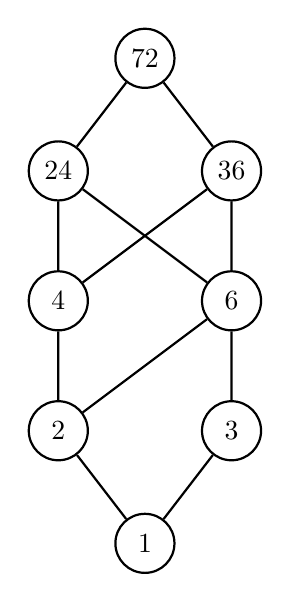
\begin{tikzpicture}[
                scale=1.1,
                every node/.style={
                    circle,
                    draw,
                    thick,
                    minimum size=7.5mm,
                    inner sep=1pt
                }
            ]
                % Вершины диаграммы Хассе по уровням
                \node (n1) at (0, 0) {$1$};
                \node (n2) at (-1, 1.3) {$2$};
                \node (n3) at (1, 1.3) {$3$};
                \node (n4) at (-1, 2.8) {$4$};
                \node (n6) at (1, 2.8) {$6$};
                \node (n24) at (-1, 4.3) {$24$};
                \node (n36) at (1, 4.3) {$36$};
                \node (n72) at (0, 5.6) {$72$};

                % Рёбра отношения покрытия (снизу вверх)
                \draw[thick] (n1) -- (n2);
                \draw[thick] (n1) -- (n3);
                \draw[thick] (n2) -- (n4);
                \draw[thick] (n2) -- (n6);
                \draw[thick] (n3) -- (n6);
                \draw[thick] (n4) -- (n24);
                \draw[thick] (n4) -- (n36);
                \draw[thick] (n6) -- (n24);
                \draw[thick] (n6) -- (n36);
                \draw[thick] (n24) -- (n72);
                \draw[thick] (n36) -- (n72);
            \end{tikzpicture}
            \caption{Диаграмма Хассе частично упорядоченного множества 
            $A = (\{1, 2, 3, 4, 6, 24, 36, 72\}, \vdots)$.}
        \end{figure}
    \end{quote}
\end{proof}

\begin{problem}
    Построить диаграмму Хассе частично упорядоченного множества 
    $B = \bigl(\powerset(\{x, y, z\}), \subseteq\bigr)$ --- булеана 
    трёхэлементного множества $\{x, y, z\}$, упорядоченного по отношению 
    включения подмножеств.
\end{problem}

\begin{proof}[Решение]~\\
    \begin{quote}
        Отношение нестрогого включения $\subseteq$ на булеане любого 
        множества всегда рефлексивно ($S \subseteq S$), антисимметрично 
        ($S \subseteq T \land T \subseteq S \implies S = T$) и транзитивно 
        ($S \subseteq T \land T \subseteq W \implies S \subseteq W$).

        В булеане $\powerset(\{x, y, z\})$ всего $2^3 = 8$ подмножеств. 
        Множество $T$ покрывает множество $S$ тогда и только тогда, когда 
        $S \subset T$ и $\abs{T} = \abs{S} + 1$ ($T$ получается из $S$ 
        добавлением ровно одного элемента). Следовательно, уровни диаграммы 
        Хассе строго соответствуют мощностям подмножеств от $0$ до $3$:

        \begin{figure}[H]
            \centering
            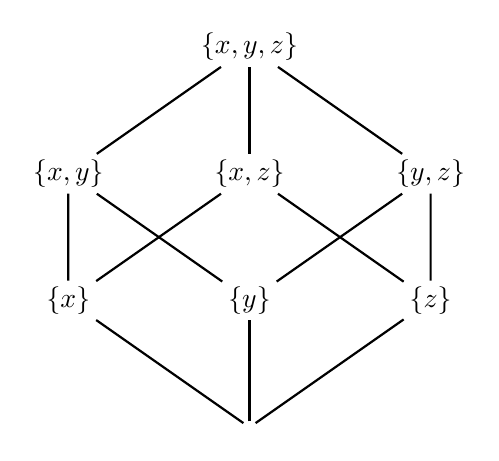
\begin{tikzpicture}[
                scale=1.15,
                every node/.style={
                    inner sep=2pt
                }
            ]
                % Уровень 0: пустое множество
                \node (empty) at (0, 0) {$\varnothing$};

                % Уровень 1: одноэлементные подмножества
                \node (x) at (-2, 1.4) {$\{x\}$};
                \node (y) at (0, 1.4) {$\{y\}$};
                \node (z) at (2, 1.4) {$\{z\}$};

                % Уровень 2: двухэлементные подмножества
                \node (xy) at (-2, 2.8) {$\{x, y\}$};
                \node (xz) at (0, 2.8) {$\{x, z\}$};
                \node (yz) at (2, 2.8) {$\{y, z\}$};

                % Уровень 3: полное множество
                \node (xyz) at (0, 4.2) {$\{x, y, z\}$};

                % Рёбра между уровнями 0 и 1
                \draw[thick] (empty) -- (x);
                \draw[thick] (empty) -- (y);
                \draw[thick] (empty) -- (z);

                % Рёбра между уровнями 1 и 2
                \draw[thick] (x) -- (xy);
                \draw[thick] (x) -- (xz);
                \draw[thick] (y) -- (xy);
                \draw[thick] (y) -- (yz);
                \draw[thick] (z) -- (xz);
                \draw[thick] (z) -- (yz);

                % Рёбра между уровнями 2 и 3
                \draw[thick] (xy) -- (xyz);
                \draw[thick] (xz) -- (xyz);
                \draw[thick] (yz) -- (xyz);
            \end{tikzpicture}
            \caption{Диаграмма Хассе булеана 
            $B = \bigl(\powerset(\{x, y, z\}), \subseteq\bigr)$ 
            (трёхмерный булев куб).}
        \end{figure}
    \end{quote}
\end{proof}

\subsubsection{Изоморфизм частично упорядоченных множеств}

\begin{definition}
    Два частично упорядоченных множества $(A, \preceq_A)$ и $(B, \preceq_B)$ 
    называются \textdef{изоморфными} (обозначается $A \cong B$), если 
    существует биективное отображение $f: A \to B$, сохраняющее отношение 
    порядка в обе стороны:
    \begin{equation} \label{eq:poset_iso}
        \forall u, v \in A : 
        \bigl(u \preceq_A v \iff f(u) \preceq_B f(v)\bigr) \tag{12}
    \end{equation}
\end{definition}

\begin{remark}[\textbf{Проверка изоморфизма по диаграммам Хассе}]
    Два конечных ЧУМ изоморфны тогда и только тогда, когда их диаграммы 
    Хассе совпадают с точностью до переименования вершин (изоморфны как 
    ориентированные снизу вверх графы).

    Сравним построенные выше восьмиэлементные ЧУМ $A$ и $B$. Несмотря на 
    одинаковое число элементов ($\abs{A} = \abs{B} = 8$), они 
    \textbf{не изоморфны} ($A \not\cong B$), что мгновенно видно по их 
    диаграммам Хассе:
    \begin{itemize}
        \item В множестве $B$ минимальный элемент $\varnothing$ покрывается 
        сразу \textbf{тремя} элементами ($\{x\}$, $\{y\}$, $\{z\}$), тогда 
        как в множестве $A$ минимальный элемент $1$ покрывается только 
        \textbf{двумя} элементами ($2$ и $3$).
        \item Длина максимальной цепи в $A$ составляет $5$ вершин 
        ($1 \to 2 \to 4 \to 24 \to 72$), а в $B$ --- только $4$ вершины 
        ($\varnothing \to \{x\} \to \{x, y\} \to \{x, y, z\}$).
    \end{itemize}
    В то же время булеан $B = \bigl(\powerset(\{x, y, z\}), \subseteq\bigr)$ 
    изоморфен ЧУМ всех натуральных делителей числа $30 = 2 \cdot 3 \cdot 5$ 
    (или любого числа $n = p_1 p_2 p_3$, являющегося произведением трёх 
    различных простых чисел) с отношением делимости.
\end{remark}

\subsubsection{Применение диаграмм Хассе в математике и информатике}

\begin{remark}[\textbf{Области применения диаграмм Хассе}]
    Диаграмма Хассе представляет собой \textdef{транзитивную редукцию} 
    конечного ориентированного ациклического графа (DAG), порождённого 
    отношением частичного порядка. Удаление рефлексивных петель и 
    транзитивных дуг позволяет компактно визуализировать и анализировать 
    сложные иерархические системы в различных областях:
    \begin{enumerate}
        \item \textbf{Теория решёток и высшая алгебра.} 
        По диаграмме Хассе мгновенно находятся \textdef{точная верхняя грань} 
        ($\sup\{x, y\} = x \lor y$, ближайшая общая вершина при движении 
        вверх) и \textdef{точная нижняя грань} ($\inf\{x, y\} = x \land y$, 
        ближайшая общая вершина при движении вниз). В алгебре с их помощью 
        строят решётки подгрупп конечной группы, решётки идеалов кольца и 
        диаграммы промежуточных полей в теории Галуа.
        \item \textbf{Планирование задач и разрешение зависимостей.} 
        В системах сборки (Make, CMake), пакетных менеджерах и планировщиках 
        процессов задачи связаны отношением «задача $A$ должна завершиться до 
        начала задачи $B$». Диаграмма Хассе отсекает избыточные транзитивные 
        зависимости, выделяет ярусы задач, которые можно выполнять 
        \emph{параллельно} (антицепи ЧУМ), и служит основой для алгоритмов 
        \textdef{топологической сортировки} (линейного доупорядочивания).
        \item \textbf{Системы типов и объектно-ориентированное 
        программирование.} 
        Отношение «тип $A$ является подтипом (наследником) типа $B$» задаёт 
        нестрогий частичный порядок. При множественном 
        наследовании диаграмма Хассе позволяет компилятору однозначно 
        определять порядок разрешения методов (MRO) и находить наименьший 
        общий надтип (Least Upper Bound) двух выражений при выводе типов.
        \item \textbf{Многокритериальная оптимизация (выбор по Парето).} 
        При сравнении объектов по нескольким признакам одновременно 
        используется покоординатный частичный порядок. Верхний 
        ярус диаграммы Хассе (множество всех максимальных элементов ЧУМ) 
        наглядно образует \textdef{фронт Парето} --- множество 
        недоминируемых альтернатив, а уровни диаграммы позволяют ранжировать 
        решения по степени их оптимальности.
        \item \textbf{Формальный анализ понятий (FCA) и защита информации.} 
        В анализе данных по бинарной матрице «объекты --- признаки» 
        строятся \textdef{решётки понятий} (диаграммы Хассе замкнутых 
        множеств признаков), используемые для иерархической кластеризации и 
        поиска ассоциативных правил. В компьютерной безопасности диаграммы 
        Хассе описывают решётку уровней допуска в мандатных моделях 
        управления доступом (модель Белла --- ЛаПадулы).
    \end{enumerate}
\end{remark}